%%%%%%%%%%%%%%%%%%%%%%%%%%%%%%%%%%%%%%%%%%%%%%%%%%%%%%%%%%%%%%%%%%%%%%%%%%%%%%%%
%characterization.tex: Chapter on ground characterization measurements:
%%%%%%%%%%%%%%%%%%%%%%%%%%%%%%%%%%%%%%%%%%%%%%%%%%%%%%%%%%%%%%%%%%%%%%%%%%%%%%%%
\chapter{Detector Characterization}
\label{characterization_chapter}
%%%%%%%%%%%%%%%%%%%%%%%%%%%%%%%%%%%%%%%%%%%%%%%%%%%%%%%%%%%%%%%%%%%%%%%%%%%%%%%%

We characterized the detectors. 

%%%%%%%%%%%%%%%%%%%%%%%%%%%%%%%%%%%%%%%%%%%%%%%%%%%%%%%%%%%%%%%%%%%%%%%%%%%%%%%%
% Parameter Measurements {{{
%%%%%%%%%%%%%%%%%%%%%%%%%%%%%%%%%%%%%%%%%%%%%%%%%%%%%%%%%%%%%%%%%%%%%%%%%%%%%%%%
\section{Detector Parameter Measurements}
\label{sec:parameter_measurements}
%%%%%%%%%%%%%%%%%%%%%%%%%%%%%%%%%%%%%%%%%%%%%%%%%%%%%%%%%%%%%%%%%%%%%%%%%%%%%%%%

%\subsection{Normal Resistance}
%TOWARDS NORMAL RESISTANCES

Given the detector design goals outlined in Section~\ref{}, as well as the limited ability to change the detector settings after the payload was launched, it was vital to carefully characterize each detector wafer before considering it for the \ac{EBEX} focal plane. 
%This section provides an overview of the characterization measurements, the sensitivity predictions, and the measured sensitivity of the detectors at float. Additional detail can be found in \cite{aubin_thesis} \cite{MacDermid_thesis} \cite{MacDermid_SPIE2014}.
Of the more than four dozen detector wafers fabricated and characterized, only 14 were able to make the final cut and earn a prized spot in the \ac{EBEX} focal plane for the \ac{EBEX2013} flight. 

For characterization measurements, we mounted the wafer, Section~\ref{}, coupled it to the readout electronics, Section~\ref{}, and cooled it to sub-Kelvin temperatures, where the exact temperature depended on the testbed. 
%highlight the difference between the light and dark configuration (and that you were attempting to minimize such that they were tested under conditions as similar to operation as possible.
The three testbeds used were: a dedicated \ac{EBEX} test cryostat at the University of Minnesota, a test cryostat at McGill University, and the \ac{EBEX} cryostat itself, made dark. 

Figure~\ref{} is a network analysis for a single comb of 16 detectors. 
The network analysis swept a voltage across the comb in frequency and measured the current response of the circuit. 
The multiplexed RLC circuit peaked in current at each LC resonant frequency. 
Around 800~mK, when the niobium leads and aluminum wirebonds were superconducting, fitting the peak width provided the normal resistance of the \ac{TES}. 
The current peak is modeled as a Lorentzian, . 
Each peak is fit individually to a Lorentzian (INCLUDE EQUATION) in order to determine each detector's resonant frequency, which is used to provide the bias signal to the TES. 
The network analysis comb is also fit to a model (INCLUDE EQUATION) to get the stray resistance and inductance in series with the comb. 

\begin{figure}[ht!]
\centering
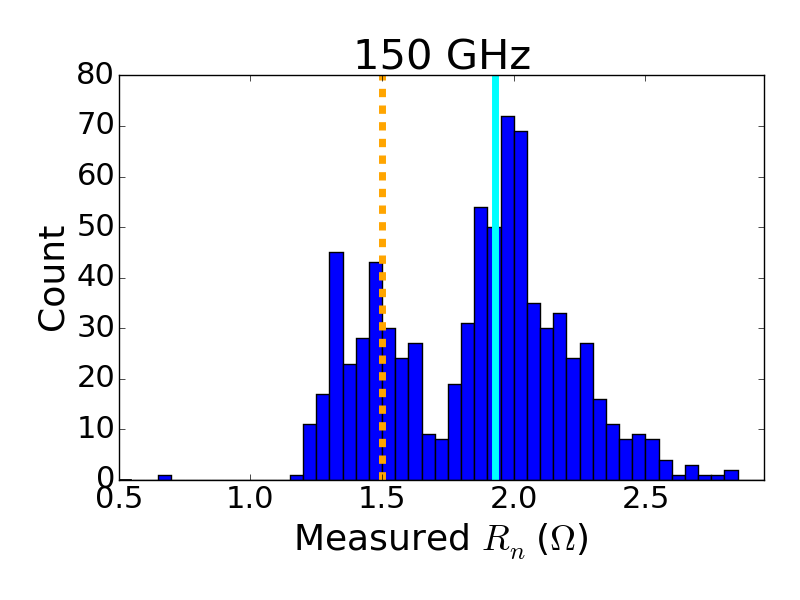
\includegraphics[width=0.31\textwidth]{figures/150_rn_hist.png}
\includegraphics[width=0.31\textwidth]{figures250_rn_hist.png}
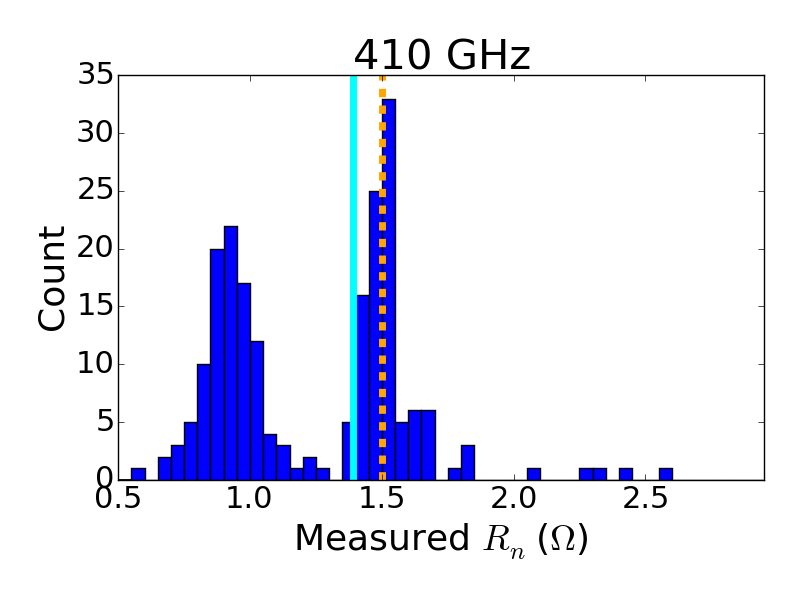
\includegraphics[width=0.31\textwidth]{figures/410_rn_hist.png}
\caption{Histogram of measured normal resistances $R_{n}$ for each of the frequency bands, including the median (vertical cyan)  
and design (\comgreen{vertical gold dashed}) values.
}
\label{fig:rn_histograms}
\end{figure}

%\subsection{Critical Temperatures}
%TOWARDS CRITICAL TEMPERATURES

\begin{figure}[ht!]
\centering
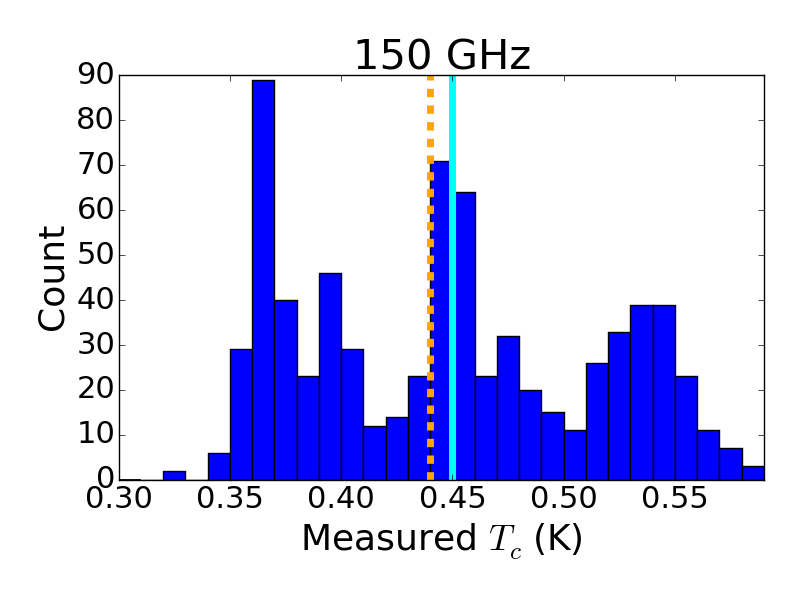
\includegraphics[width=0.31\textwidth]{figures/150_tc_hist.png}
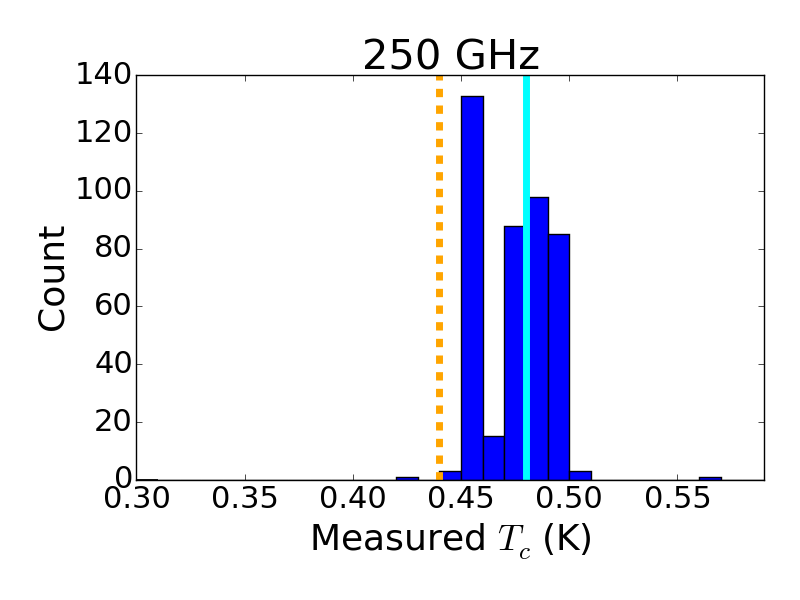
\includegraphics[width=0.31\textwidth]{figures/250_tc_hist.png}
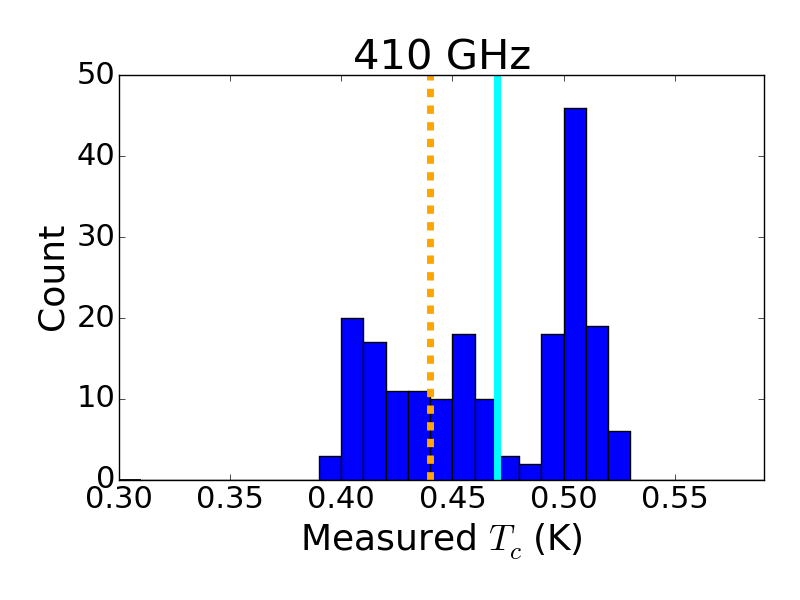
\includegraphics[width=0.31\textwidth]{figures/410_tc_hist.png}
\caption{Histogram of measured critical temperature values for the detectors in each frequency band including the median (vertical cyan) and design (vertical gold dashed) values. 
\label{fig:tc_histograms} }
\end{figure}

%\subsection{Thermal Conductances}
%TOWARDS THERMAL CONDUCTANCES 

\begin{figure}[ht!]
\centering
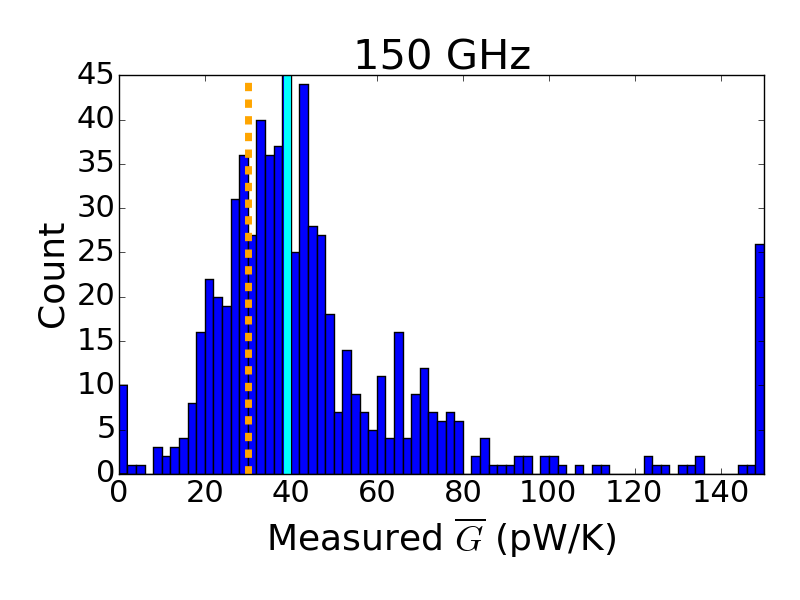
\includegraphics[width=0.31\columnwidth]{figures/150_g_bar_hist.png}
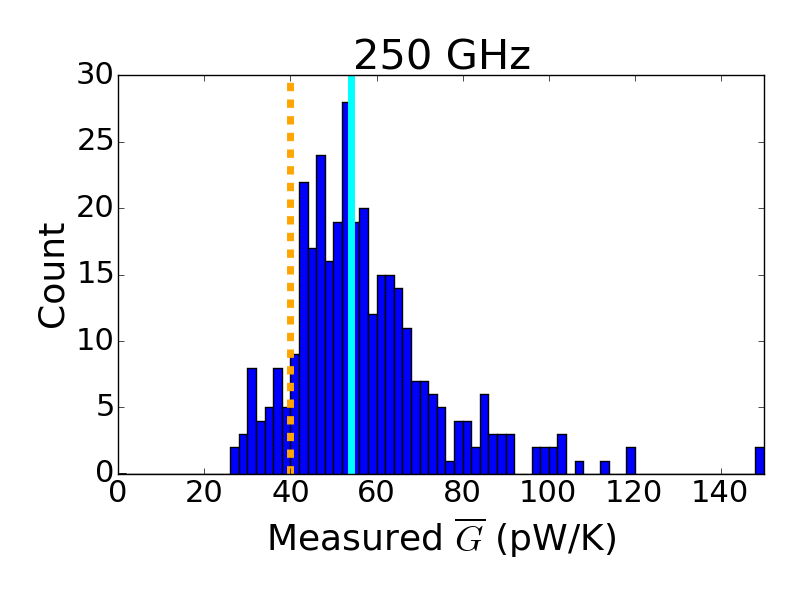
\includegraphics[width=0.31\columnwidth]{figures/250_g_bar_hist.png}
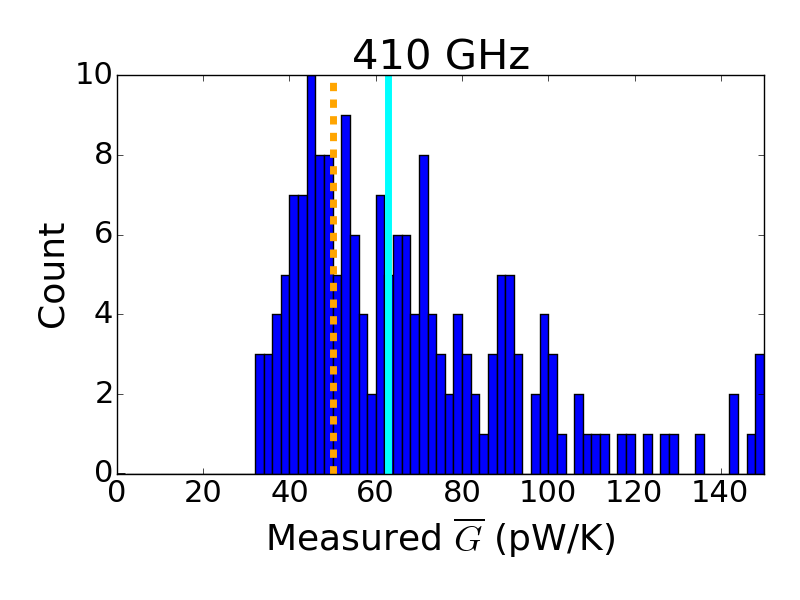
\includegraphics[width=0.31\columnwidth]{figures/410_g_bar_hist.png}
\caption{Histograms of the measured average thermal conductance values for the three frequency bands including the 
median (vertical cyan) and design (vertical gold dashed) values. 
We piled measurements of  $\overline{G}$ exceeding 150~pW/K into the last histogram bin.
%\comred{these histograms have values in excess of 150 pW/K piled in the last bin, but other histograms (throughout paper) don't do this. Should I re-make without piling?}
}
\label{fig:G_Histograms} 
\end{figure}


%%%%%%%%%%%%%%%%%%%%%%%%%%%%%%%%%%%%%%%%%%%%%%%%%%%%%%%%%%%%%%%%%%%%%%%%%%%%%}}}

%%%%%%%%%%%%%%%%%%%%%%%%%%%%%%%%%%%%%%%%%%%%%%%%%%%%%%%%%%%%%%%%%%%%%%%%%%%%%%%%
% Optical Efficiency {{{
%%%%%%%%%%%%%%%%%%%%%%%%%%%%%%%%%%%%%%%%%%%%%%%%%%%%%%%%%%%%%%%%%%%%%%%%%%%%%%%%
\section{Optical Efficiency}
\label{sec:optical_efficiency}
%%%%%%%%%%%%%%%%%%%%%%%%%%%%%%%%%%%%%%%%%%%%%%%%%%%%%%%%%%%%%%%%%%%%%%%%%%%%%%%%

\begin{figure}[ht!]
\begin{center}
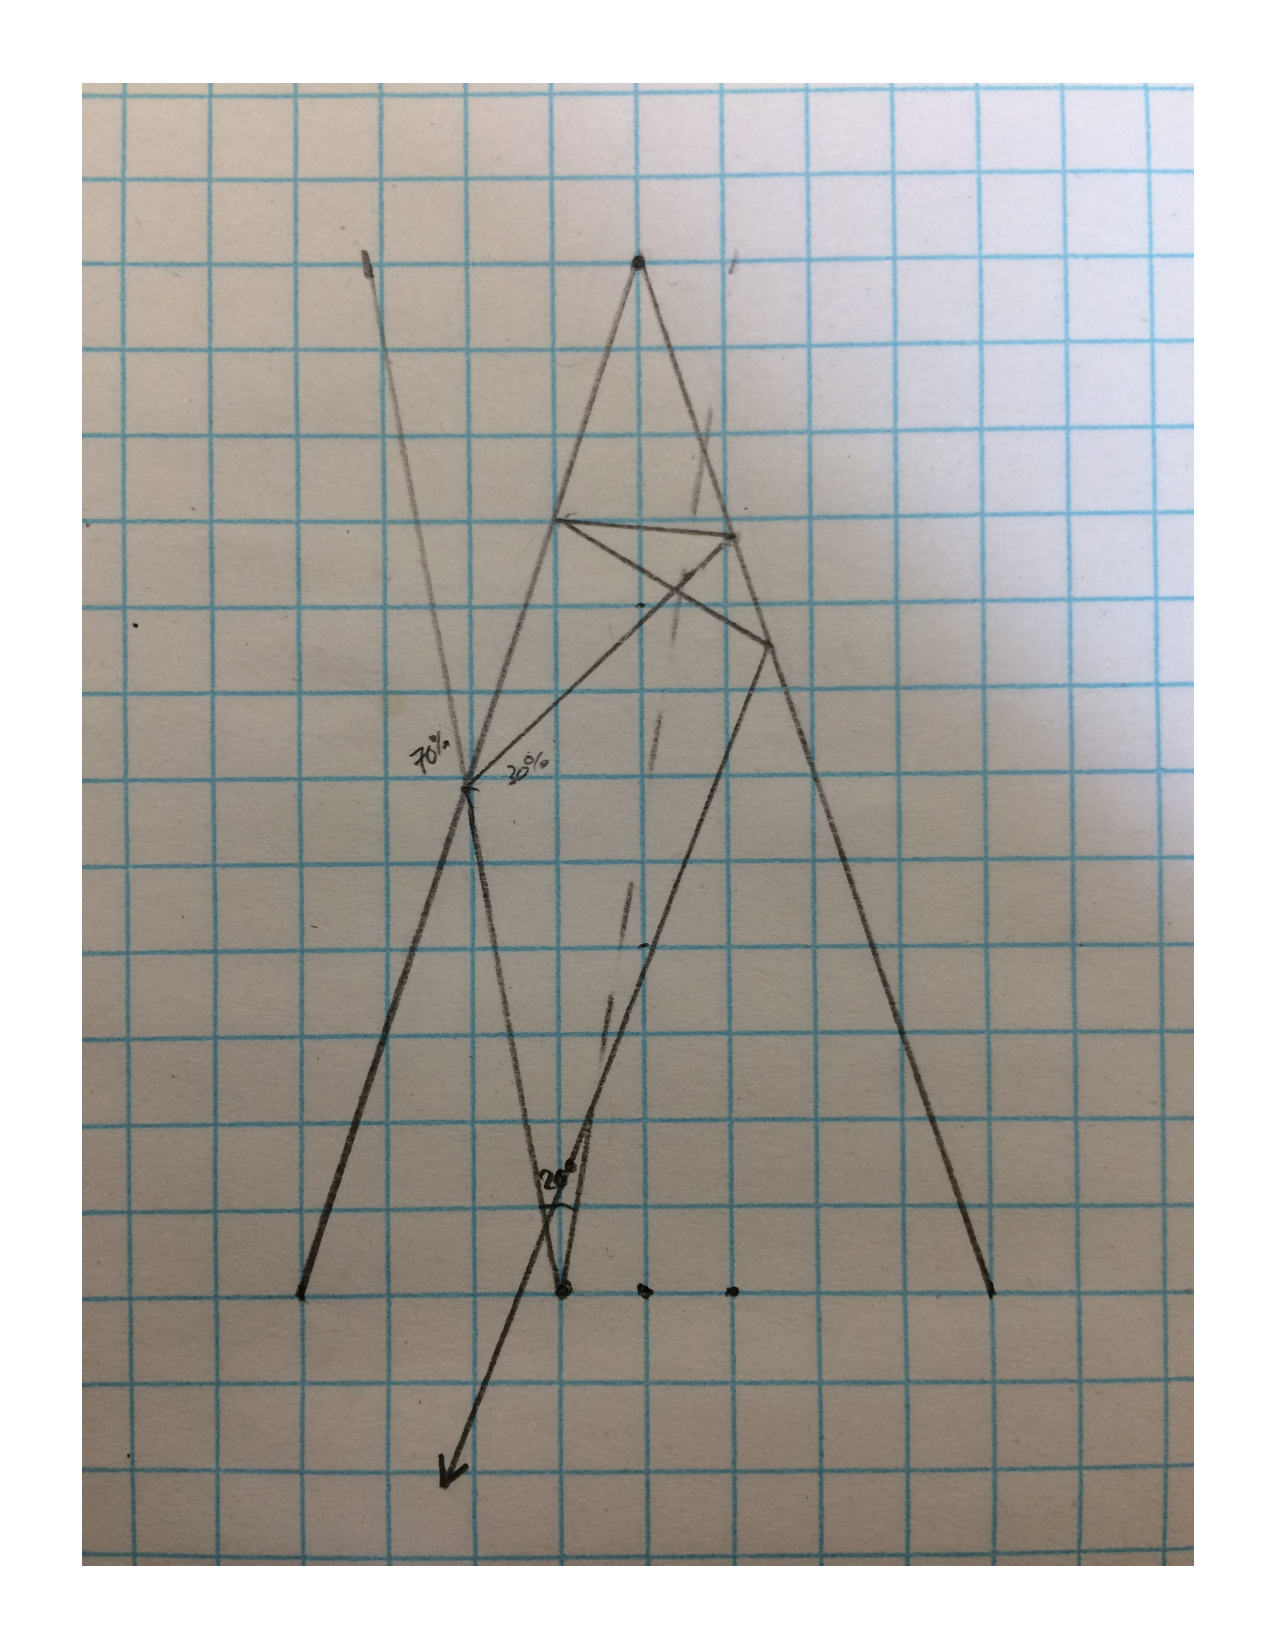
\includegraphics[height=2.5in]{figures/blackbody_design2}
\caption{Eccosorb blackbody design. 
\label{fig:blackbody_design} }
\end{center}
\end{figure}

\begin{figure}[ht!]
\begin{center}
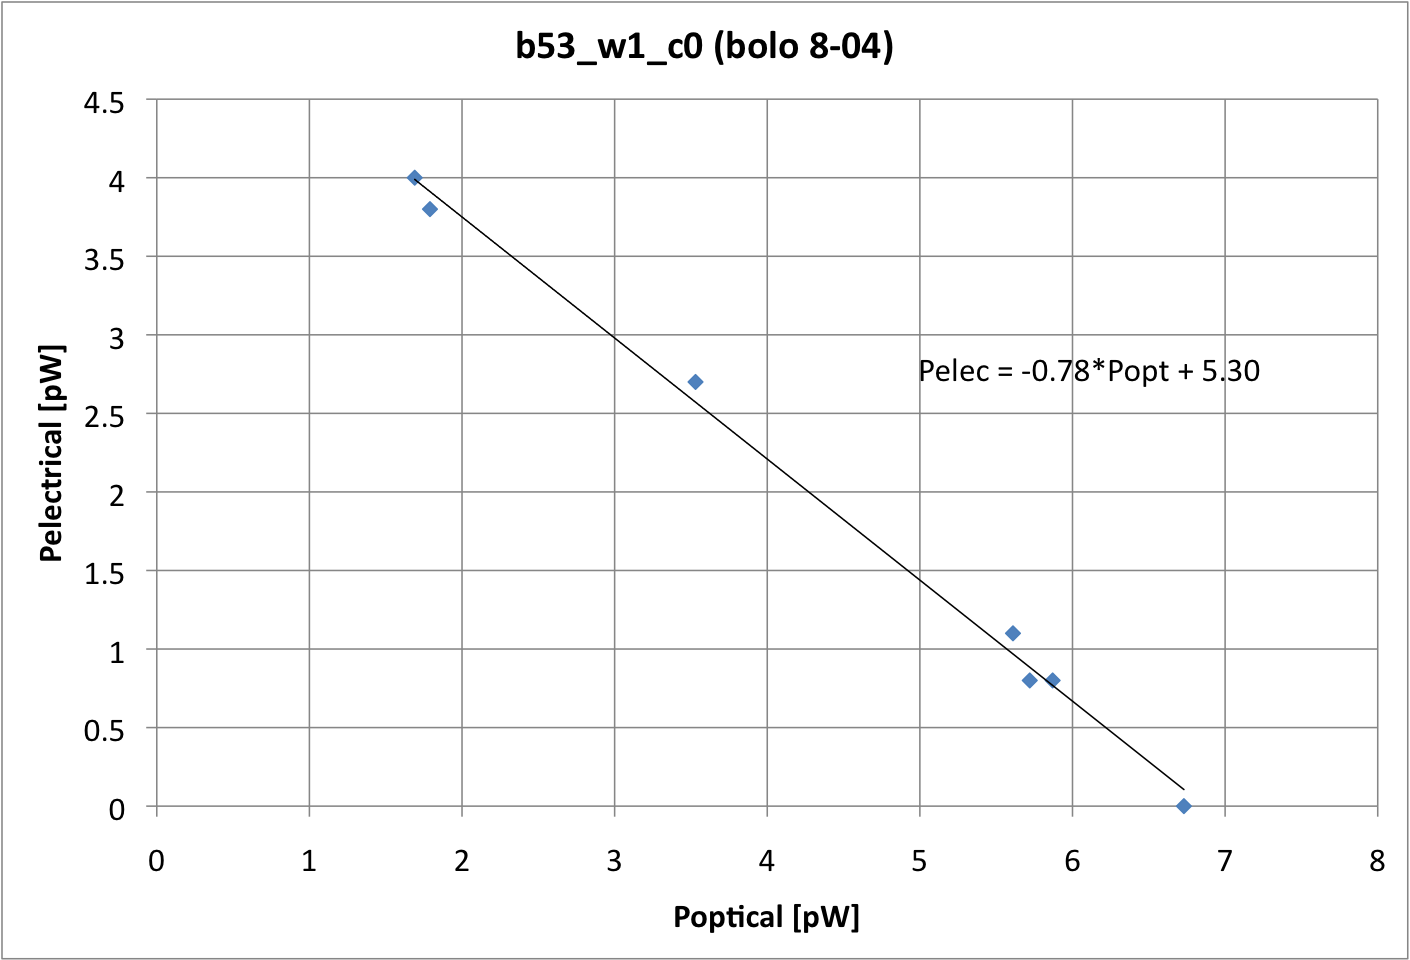
\includegraphics[height=2.5in]{figures/Nb01_PelecvsPopt_b53_w1_c0}
\caption{One 150-01 detector electrical power as function of blackbody power. The slope is the detector's optical efficiency. 
\label{fig:pelec_vs_popt} }
\end{center}
\end{figure}


\begin{figure}[ht!]
\begin{center}
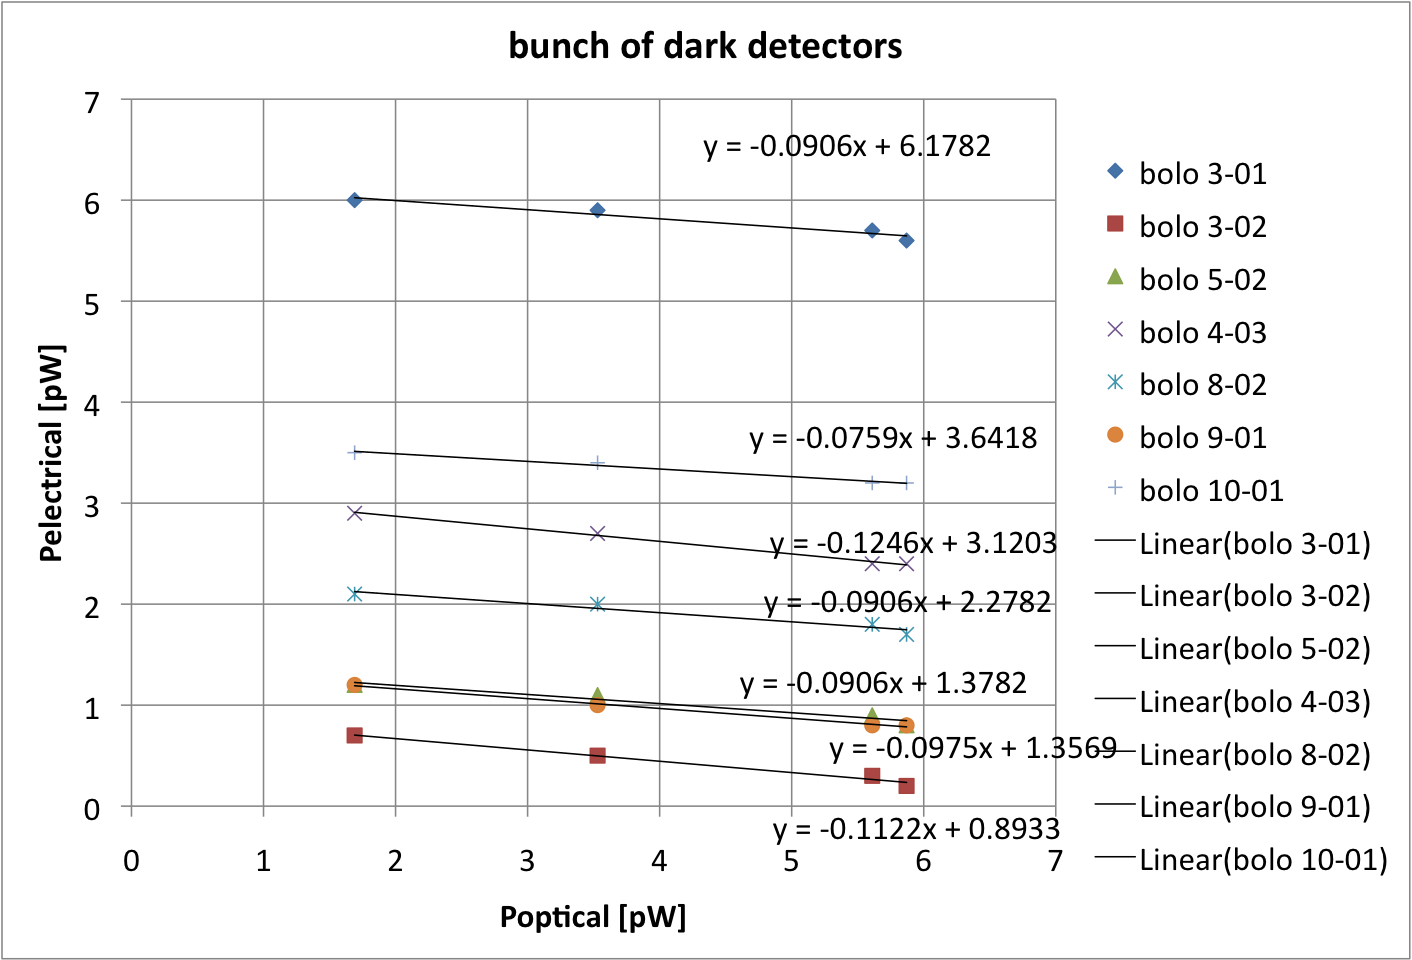
\includegraphics[height=2.5in]{figures/darkdetectoreffs}
\caption{The dark detectors also observed a decrease in electrical power needed to keep the detector in the transition as the black body temperature was turned up. The slope of this line gives the "efficiency" of the dark detectors. Some measure of the level of optical cross talk?
\label{fig:dark_optical_efficiencies} }
\end{center}
\end{figure}


%%%%%%%%%%%%%%%%%%%%%%%%%%%%%%%%%%%%%%%%%%%%%%%%%%%%%%%%%%%%%%%%%%%%%%%%%%%%%}}}


%%%%%%%%%%%%%%%%%%%%%%%%%%%%%%%%%%%%%%%%%%%%%%%%%%%%%%%%%%%%%%%%%%%%%%%%%%%%%%%%
% Dark Noise Performance {{{
%%%%%%%%%%%%%%%%%%%%%%%%%%%%%%%%%%%%%%%%%%%%%%%%%%%%%%%%%%%%%%%%%%%%%%%%%%%%%%%%
\section{Dark Noise Performance}
\label{sec:dark_nosie}
%%%%%%%%%%%%%%%%%%%%%%%%%%%%%%%%%%%%%%%%%%%%%%%%%%%%%%%%%%%%%%%%%%%%%%%%%%%%%%%%


\begin{figure}[ht!]
\begin{center}
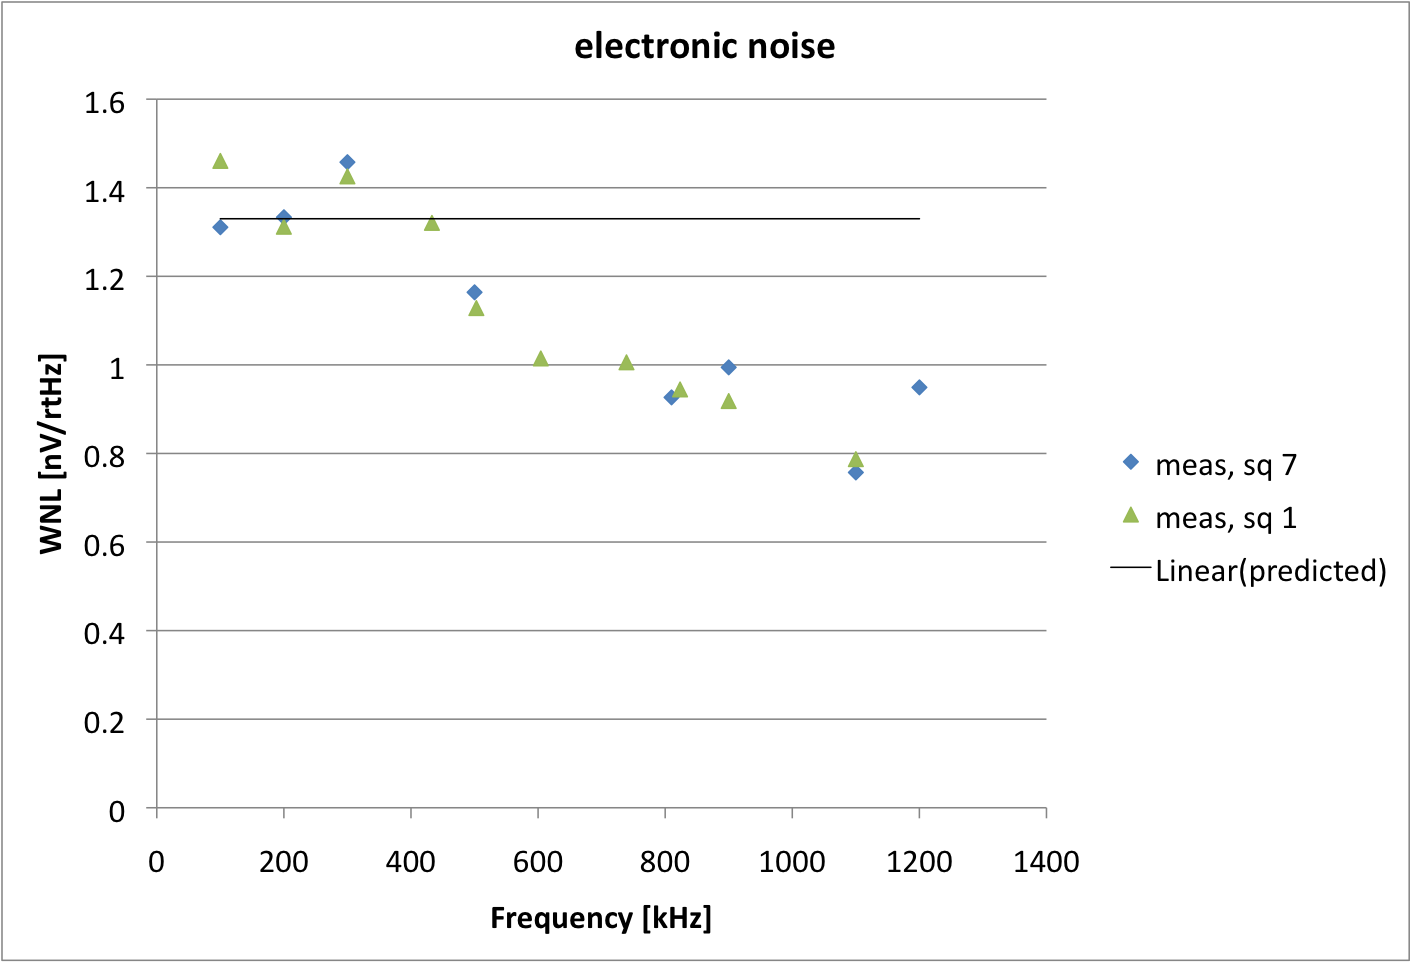
\includegraphics[height=2.5in]{figures/electronic_noise_sq1_sq7}
\caption{Electronic noise of warm electronics in \ac{ETC}. Units of $nV/\sqrt{Hz}$. This is probing the system from point A to point B. It includes the noise of ... .
\label{fig:dark_electronic_noise} }
\end{center}
\end{figure}

\begin{figure}[ht!]
\begin{center}
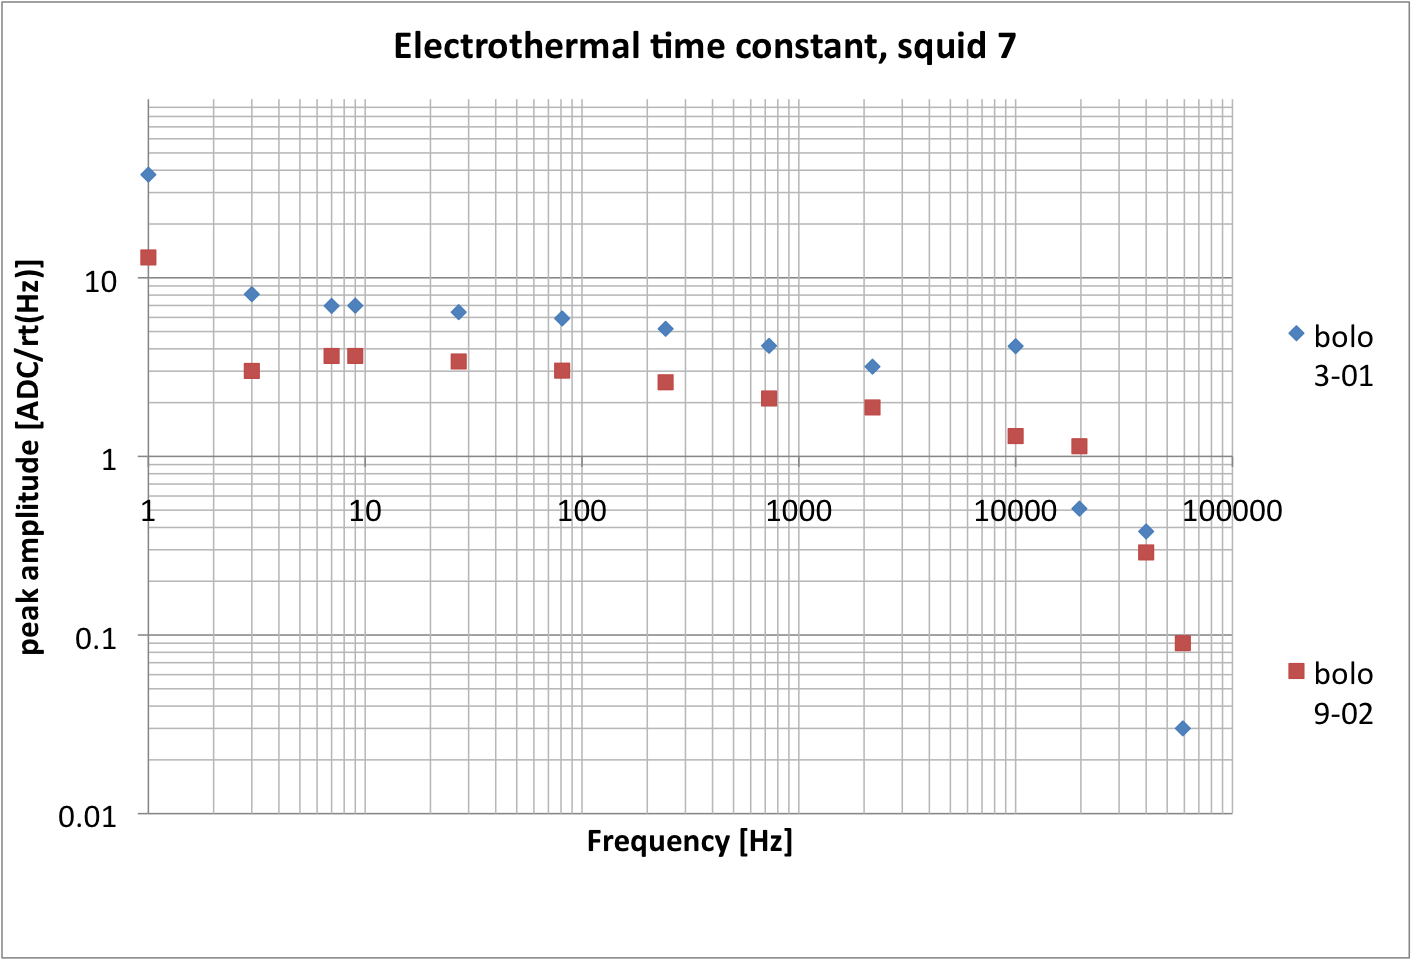
\includegraphics[height=2.5in]{figures/Nb01_squid7_etau_morepts}
\caption{Electrothermal time constants of two bolometers on 150-01. What does the fit to this data give? This is the time constant between the TES and the web? As expected, the for the web to thermalize is much faster than the optical time constant (time for light to couple to the web). 
\label{fig:electrothermal_tau} }
\end{center}
\end{figure}

\begin{figure}[ht!]
\begin{center}
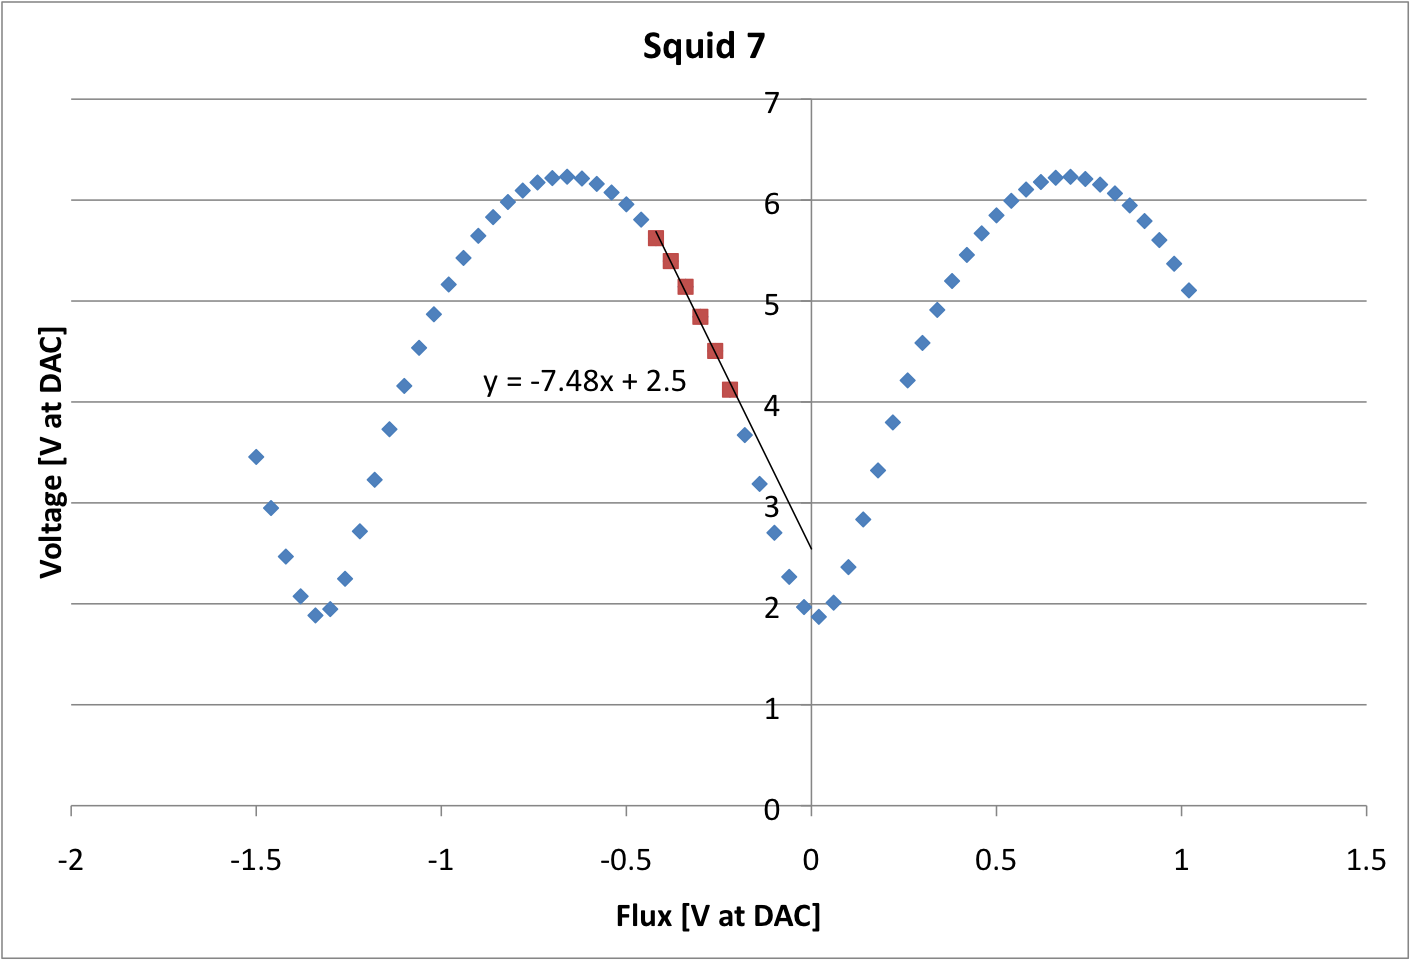
\includegraphics[height=2.5in]{figures/squid7_transimp}
\caption{\ac{SQUID} voltage versus current/flux curve. Operating regime is highlighted. Transimpedance, $dV/d\phi$ is the slope of the line.
\label{fig:squid_transimpedance} }
\end{center}
\end{figure}

\begin{figure}[ht!]
\begin{center}
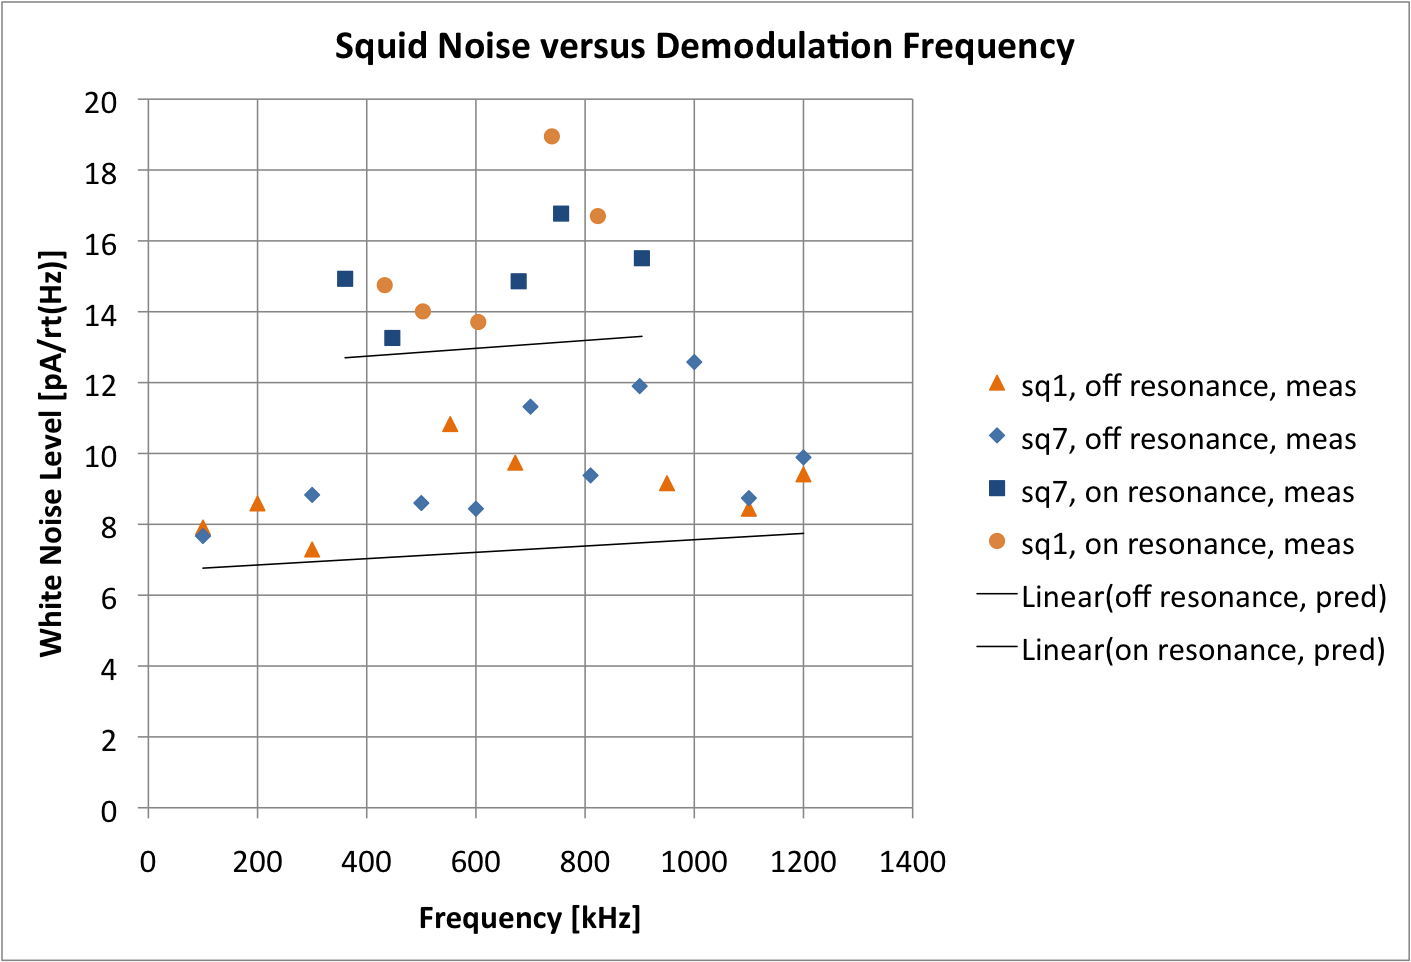
\includegraphics[height=2.5in]{figures/squidnoise_temp}
\caption{\ac{SQUID} noise in \ac{ETC} as function of demodulation frequency. At detector demodulation frequencies, the Johnson noise term of the bolometer roughly doubles the noise.
\label{fig:dark_squid_noise} }
\end{center}
\end{figure}



%%%%%%%%%%%%%%%%%%%%%%%%%%%%%%%%%%%%%%%%%%%%%%%%%%%%%%%%%%%%%%%%%%%%%%%%%%%%%}}}
